

Woodcutting focuses on collecting logs by chopping them with a given axe. The main modifiers to experience are the type of axe and the type of tree. In Fig.~\ref{fig:woodcutting_landscape} you can see an experience landscape that shows the experience rate per hour based on the tree (by level, eg: 15 is oak) and wooductting level. For this section, a small dataset was collected to measure various tree chop rates at a few levels. The rates are interpolated to work for any level. 


Each tree requires data to be collected at two points and a linear interpolation can be used to determine the rate at any level. The sample was collected on two accounts at level 45 and 77 woodcutting. Since trees above 45 cannot be cut, they represented extrapolated values. Since the highest level that can analyzed by this data collection is 45, parts of the landscape aren't possible (eg: chopping Oak at level 1).

\begin{figure}
	\centering
	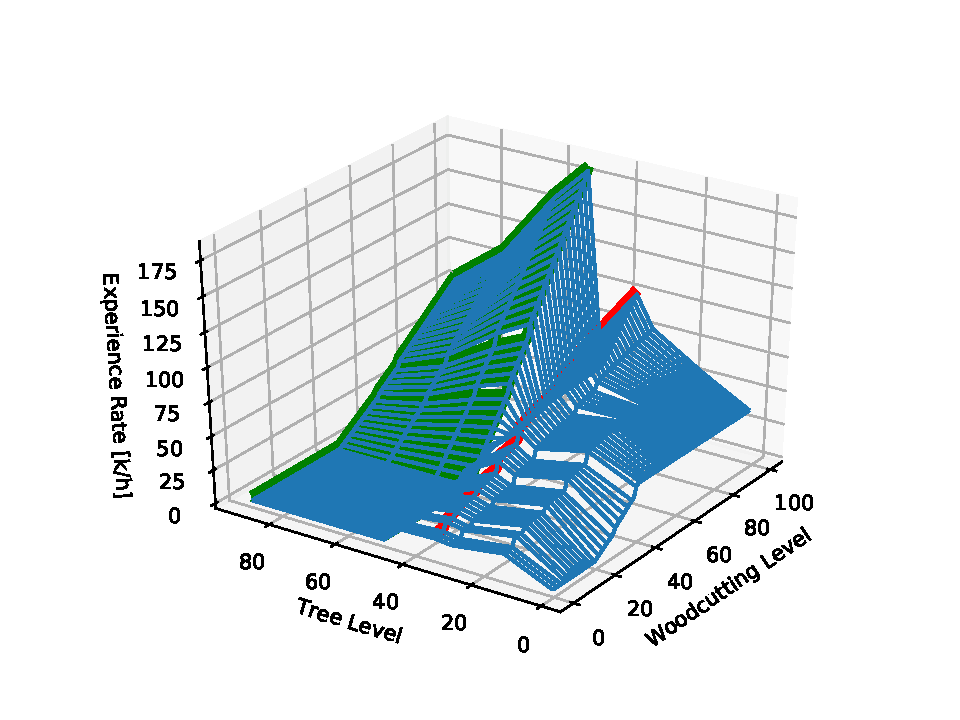
\includegraphics[width=\linewidth]{img/woodcutting/experience.pdf}
	\caption{
		The experience levels for \emph{Teak Trees} in red are exactly known and not estimated by a sample. The portion in green represents extrapolations out side of the dataset (due to the 45 woodcutting limitation). As a result the extrapolations near $L=50$ are misleading. 
	}
	\label{fig:woodcutting_landscape}
\end{figure}


For more details, you can watch the \href{https://www.youtube.com/watch?v=vYPLkFTDe5Y&t=39s&ab_channel=Palfore}{Optimizing Runescape Woodcutting Video}. Furthermore, the wiki team has recently provided a complete and comprehensive set of values in the \href{https://oldschool.runescape.wiki/w/Pay-to-play_Woodcutting_training\#Theoretical_experience_rates}{Theoretical Woodcutting XP Rates} page which now supersedes this work.
